\chapter{Introduction}

\section{Introduction}
In last few years, growth in web technologies, Artificial Intelligence (AI), and Machine Learning (ML), with the availability of the Internet, have changed how people online shopping for products . Previously shopping is often limited by store location, inventory constraints, and long communication between customers and sales staff. Now a days, modern consumers increasingly expect convenience, personalized recommendations, and quick access to relevant products across a wide range of categories.

Bangladesh’s uprising bond with the global retail and technology sector,with increasing local interest in virtual-online businesses, has created a Desire for scalable e-commerce solutions. However, most of the small and medium-sized businesses still not have the technical infrastructure to build their own online e-commerce platforms. They mainly depends on basic web shops or social media pages that do not provide advanced search, recommendation, or analytics capabilities. As a result, customers find it hard to quickly find suitable products, compare alternatives, or receive meaningful guidance without going to the physical stores.

Some research on online retail point out that seamless digital interactions and reduced friction while browsing and checkout are critical for retaining customers and improving sales performance\cite{lee2020checkout}. On the other hand, other researches on digital and mobile financial services point out the importance of offering multiple secure and convenient payment options such as bank cards and mobile wallets(MFS) to increase user trust and promote online transaction adoption in developing countries \cite{hasan2021mobile}. In Bangladesh, mobile financial services like bKash have become widely accepted, yet many smaller e-commerce sites still not willing to integrate these services into their sites for a unified, automated shopping experience.


To resolve these challenges and problems, our project introduces \textit{ShopSense: Intelligent E-Commerce Platform}, an AI-enhanced online shopping system that solves the challenges and provide a traditional e-commerce workflow with intelligent search, recommendation, and chat support. The platform helps customers to browse products, apply filters, ML-driven recommendations, interact with the chat-bot(RAG), manage their cart, complete secure payments, and track orders. Admin/Shop-Owner can manage products, categories, coupons, and orders using dedicated backend interface, supported by analytics derived from user interactions.

ShopSense is developed using Django for the backend, HTML/CSS and modern web tools for the front-end, and a relational database for a reliable data storage. AI and ML components are used to generate product embeddings, power semantic search, and uses  user behavior to continuously improve recommendation and user experience. By combining these technologies, the system aims to reduce traditional processes, improve product relevance, support multiple payment system (including local gateways), and provide a better, data-driven shopping experience for customers and store owners.

\section{Motivation}
In this growing digital commerce environment, many small and medium-sized online stores still depends on partially manual processes for order placement and payment. For example, platforms like \href{https://ghorerbazar.com}{ghorerbazar.com} require or prefer customers to contact the seller manually (e.g., phone calls or messaging apps) to confirm orders and mainly support Cash on Delivery (COD) as the payment method. This process can introduce some friction, delays, and a risk of miscommunication, and it can make the ability to scale or automate business operations and need manpower to operate smoothly.

Few previous studies show that each additional click or interruption in the checkout process can increase users leaving and possibly reduce user satisfaction \cite{lee2020checkout}. When customers are  kind of forced to leave the website to complete an order or payment arrangement, they are more likely to abandon the purchase or switch to competitors that provide a seamless end-to-end flow \cite{lee2020checkout,hasan2021mobile}. Only cash-on-delivery can make logistics more complex, and there is a higher probability of refusing deliveries, which can cause small businesses to collapse as they have limited capacity for operations\cite{rahman2018cod}.


Supporting multiple payment options, such as card payments or mobile financial services, is proven by research to convince people to adopt online payments in developing economies  \cite{hasan2021mobile}. In markets like Bangladesh, mobile financial services, such as bKash, have already become a part of everyday financial activity, and integrating them directly into e-commerce platforms can substantially increase user trust and transaction volume  \cite{hasan2021mobile}. Platforms that rely only on manual payments or cash on delivery (COD) may fail to take advantage of these developments and remain vulnerable to inefficiencies and loss of revenue \cite{rahman2018cod}. 
In this project, we will attempt to develop a system that can reduce manual steps, introduce multiple payment methods, and bring artificial intelligence (AI) to enhance customer service and product discovery while remaining straightforward and deployable for Bangladeshi small and medium-sized businesses. 

\section{Objectives of the Project}
Our main goal for this project is to create and deploy an intelligent e-commerce platform that offers a seamless online shopping experience for both customers and store administrators. In order to accomplish this overall goal, the project aims to meet the following specific objectives: 

\begin{itemize}
  \item To construct a full-featured e-commerce web application that allows product browsing, cart management, checkout, and order tracking within a single online interface. 
  \item To include several payment alternatives, such as card payments (via Stripe), mobile banking (via bKash), to eliminate manual management and cash-on-delivery only workflows \cite{hasan2021mobile}.
  \item To design and deploy AI-based semantic search that allows customers to find relevant products using natural language queries and similarity-based retrieval;
  \item To implement a recommendation engine that provides personalized product suggestions based on product content and user interaction history;
  \item To build an AI chatbot that can answer product-related queries,remember context, assist with order information, and derive customers through the shopping process;
  \item To provide an admin backend for managing products, categories, coupons, users, and orders, along with basic analytics derived from transactional and interaction data.
\end{itemize}

\section{Project Scope}
The scope of this project is intentionally focused on building a practical, deployable prototype of an AI-enhanced e-commerce platform rather than a complete commercial system. The major components included within the scope are:

\begin{itemize}
  \item Design and implementation of a web-based storefront where customers can register, log in, browse products by category, view details, manage a shopping cart, and place orders;
  \item Development of core backend services in Django, including models for products, categories, users, orders, payments, and coupons, as well as RESTful APIs for frontend integration;
  \item Integration of Stripe and bKash payment gateways in sandbox or test mode, alongside a mock payment gateway for development and demonstration purposes;
  \item Implementation of AI and ML components for semantic search, product recommendations, and chatbot assistance using appropriate libraries and tools;

  \item Creation of an admin dashboard for order processing, promotions, and catalog data management utilizing Django's admin panel and/or custom views.

  \item A simple deployment setup that will provide information about utilizing a cloud-friendly configuration, such as Render, Railway, or a comparable platform. 
\end{itemize}

Some elements are outside the scope of this project, including:
 \begin{itemize}
  \item Complex multi-vendor marketplace features, such as seller portals or revenue sharing;

  \item Full-scale production hardening, such as extensive security audits, high-availability infrastructure, or large-scale performance optimization.
\end{itemize}

\section{Project Contribution}

In the context of intelligent commercial systems, this project makes various methodological and practical contributions:


\begin{itemize}
  \item It shows how various payment methods, such as credit/debit cards, mobile banking, and COD, can be integrated to reduce checkout friction and encourage online transaction adoption in developing countries.
  \item It presents a unified architecture that combines a traditional online-commerce workflow with AI-driven search, recommendations, and conversational assistance tailored for small and medium-sized merchants \cite{hasan2021mobile,rahman2018cod}.
  \item It demonstrates a practical chatbot integration that uses retrieval-augmented generation to answer product and order-related queries naturally and contextually.
  \item It offers documentation, configuration guidelines, and example datasets helpful for students, researchers, and developers exploring AI-enhanced e-commerce applications.
  \item It offers a usable implementation of semantic search and recommendation features adaptable to similar retail domains.
\end{itemize}

The project shows how interaction and transaction data can be formatted to facilitate analytics, such as identifying popular products, user behavior trends, and promotion efficacy, in addition to these technological contributions \cite{lee2020checkout}.

\section{Gantt Chart}
The development of ShopSense was planned over several phases spanning approximately sixteen weeks, from early March to late October. The high-level timeline is illustrated in Figure~\ref{fig:gantt-chart}, which shows the main phases of work and their approximate durations:

\begin{itemize}
  \item \textbf{Task 1: Planning \& Setup (Mar -- May)}: Requirements analysis and literature review, and system design.
  \item \textbf{Task 2: Core Development (May -- Jul)}: Implementation of authentication, user accounts, and product features.
  \item \textbf{Task 3: Advanced Features (Jun -- Sep)}: Implementation of checkout, order management, and payment integration.
  \item \textbf{Task 4: AI/ML Implementation (Jul -- Oct)}: Development of semantic search, recommendations, and chat-bot integration.
  \item \textbf{Task 5: Testing \& Deployment (Sep -- Nov)}: System testing, bug fixing, performance checks, and deployment configuration.
  \item \textbf{Task 6: Documentation (Jun -- Nov)}: Documenting of each feature for project report.
\end{itemize}

\begin{figure}[H]
  \centering
  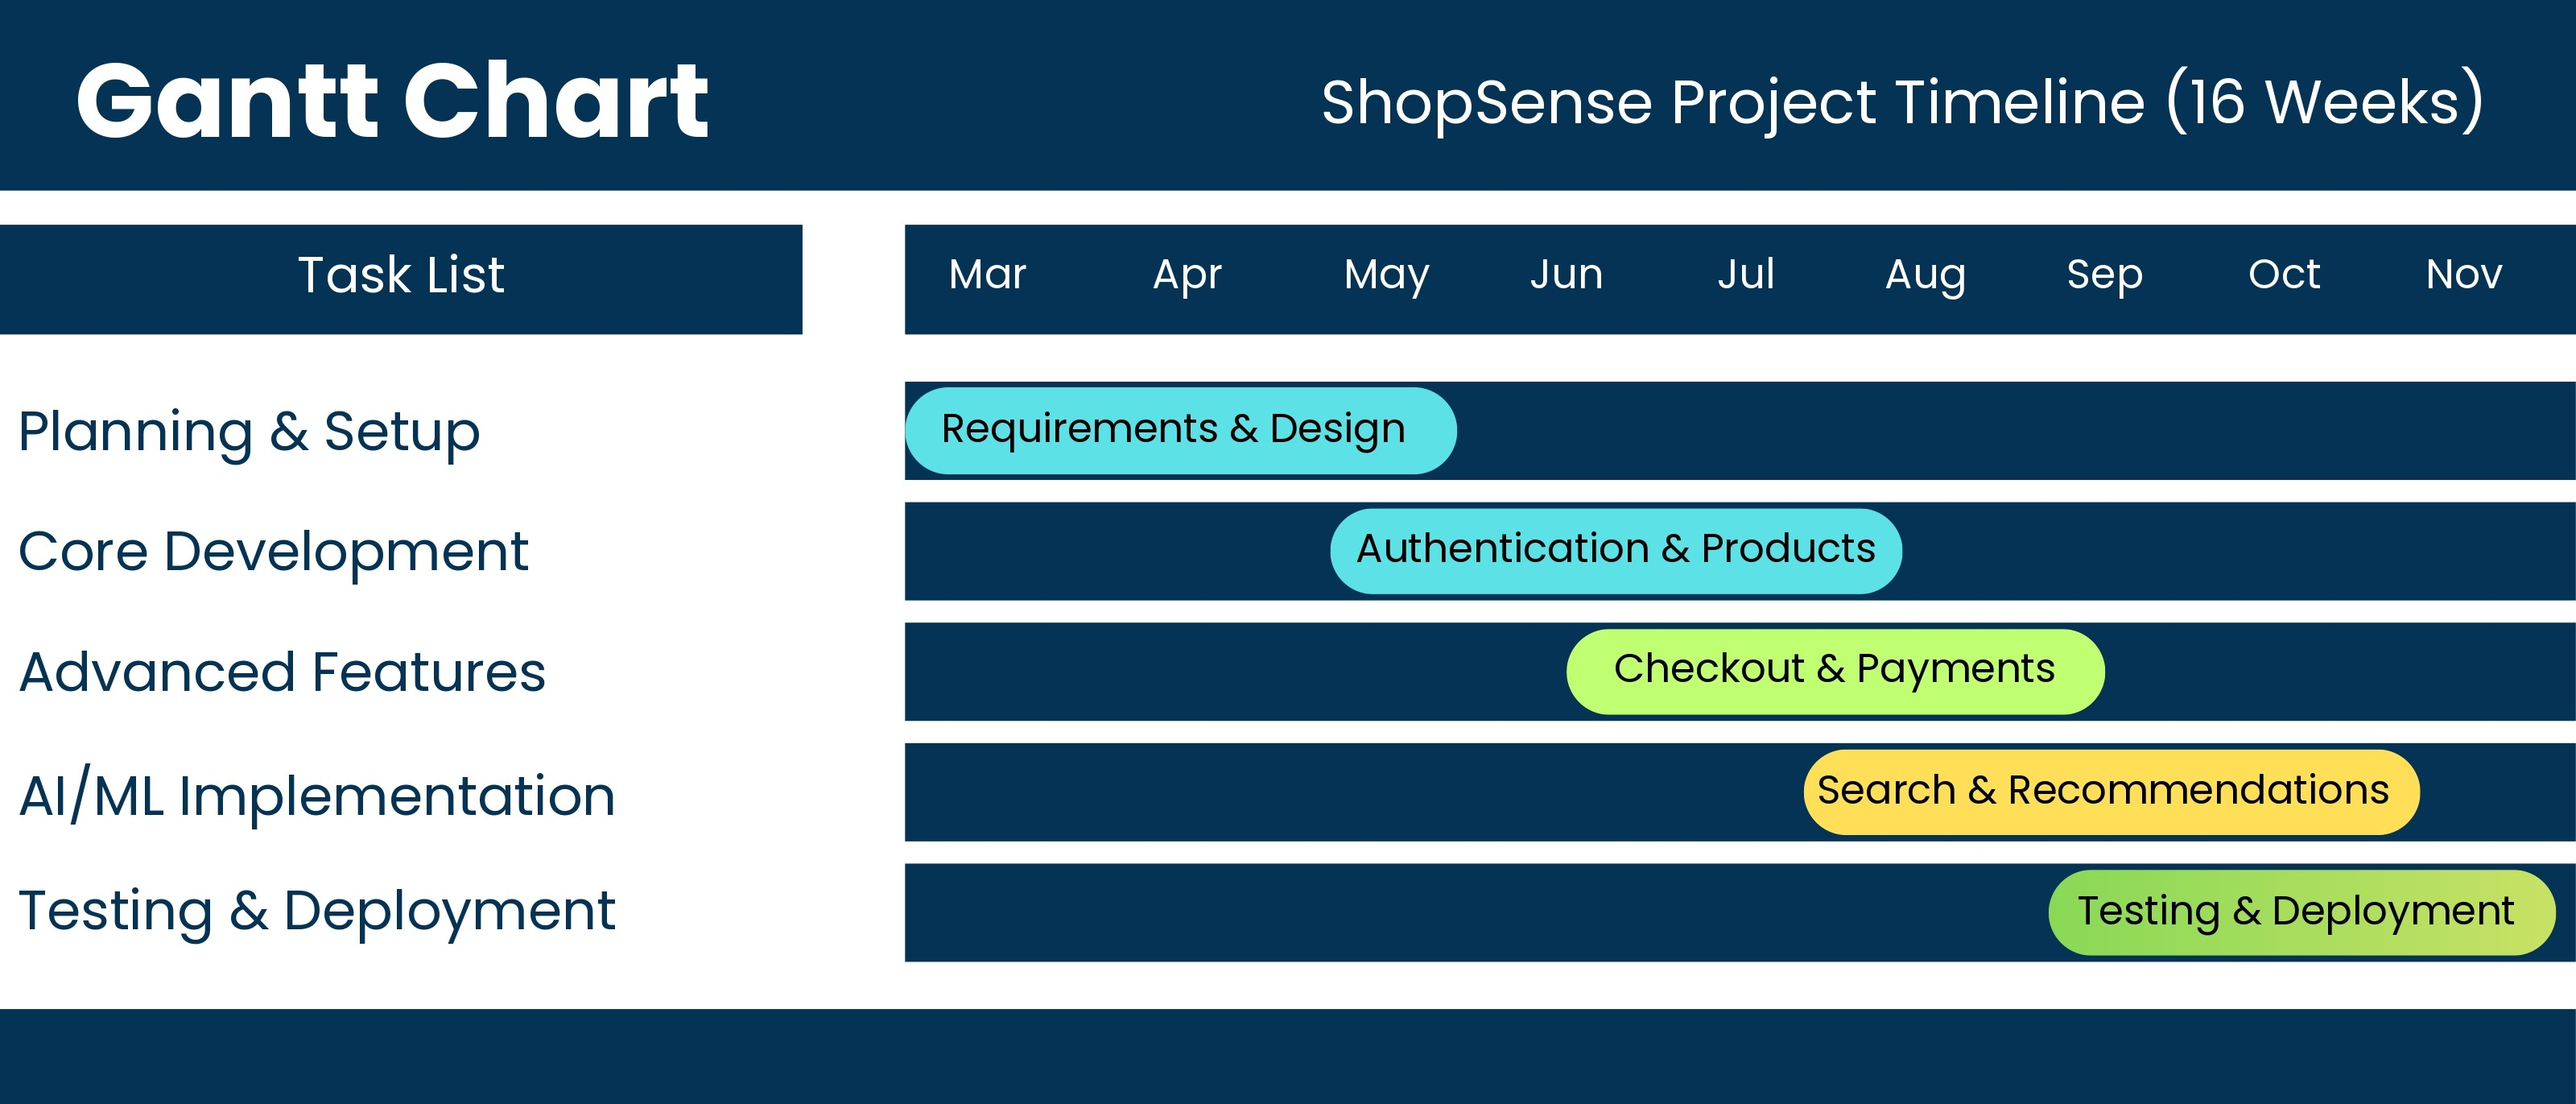
\includegraphics[width=0.95\textwidth]{Images/MyFigs/ShopSense Gantt Chart.jpg}
  \caption{ShopSense project timeline showing the main development phases over a 16-week period.}
  \label{fig:gantt-chart}
\end{figure}

\section{Budget Details}
Table~\ref{table:project_budget} shows the projected sum for the ShopSense project, calculated in Bangladeshi Taka (BDT). The budget considers human resources, software and tooling, hosting, payment gateway setup, and other supporting costs, as well as a contingency allocation.


\begin{table}[H]
\centering
\caption{ShopSense project budget summary.}
\begin{tabular}{|l|r|}
\hline
\textbf{Category} & \textbf{Cost (BDT)} \\
\hline
Human Resources / (Developer-Designer cost) & 62,000 \\
\hline
Software \& Tools & 3,500 \\
\hline
Cloud \& Hosting & 14,000 \\
\hline
Payment Gateway Setup & 5,000 \\
\hline
Domain \& SSL & 2,000 \\
\hline
Hardware \& Equipment & 5,500 \\
\hline
Miscellaneous Expenses & 6,900 \\
\hline
Contingency (10\%) & 8,900 \\
\hline
\textbf{Total Estimated Cost} & \textbf{97,900} \\
\hline
\end{tabular}
\label{table:project_budget}
\end{table}


The budget assumes moderate-scale development effort with a small team, reliance on mostly open-source technologies, and usage of affordable cloud hosting options suitable for academic or pilot deployments.
\section{Organization of the Report}
The remainder of this report is organized as follows:

\begin{itemize}
  \item \textbf{Chapter~2} presents the literature review and related work on e-commerce platforms, AI-driven search and recommendation systems, online payment integration, and mobile financial services in developing countries.
  \item \textbf{Chapter~3} describes the design methods and procedures, including the overall architecture of ShopSense, database schema, major system modules, data flow diagrams, and design considerations for AI and payment components.
  \item \textbf{Chapter~4} explains the implementation details of the ShopSense platform, covering backend and frontend development, integration of AI services, configuration of payment gateways, deployment setup, and user interface screenshots.
  \item \textbf{Chapter~5} concludes the report by summarizing the main contributions, discussing general findings, outlining limitations of the current prototype, and presenting directions for future work and practical implications.
\end{itemize}

\section{Conclusion}
This chapter introduced the background, motivation, objectives, scope, and contributions of the \textit{ShopSense} project, and outlined the structure of the remaining chapters. It also presented an overview of the project schedule and budget. The next chapter reviews related work in intelligent e-commerce, AI-driven search and recommendation, and online payment integration to position ShopSense within the broader research and industry context.